\documentclass[titlepage, a4paper]{article}
%importerat (2017-01-24) layout-bibliotek från Hannes Snögren, KMM 14/15. Med godkännande från honom. 
%ändrat i settings sedan dess. babel-bibliotek för swedish krävs för kompilering.
%debian: sudo apt-get install texlive-lang-european

\usepackage[swedish]{babel}
\usepackage[utf8]{inputenc}
\usepackage{color}
\usepackage{graphicx}
\usepackage{etoolbox}
\usepackage{hyperref}
\usepackage{calc}  
\usepackage{enumitem}
\usepackage{titlesec}

\makeatletter
\patchcmd{\ttlh@hang}{\parindent\z@}{\parindent\z@\leavevmode}{}{}
\patchcmd{\ttlh@hang}{\noindent}{}{}{}
\makeatother

%Spacing för sections och subsections
\titlespacing*{\section}
{0pt}{5.5ex plus 1ex minus .2ex}{1.0ex plus .2ex}
%\titlespacing*{\subsection}
%{0pt}{5.5ex plus 1ex minus .2ex}{4.3ex plus .2ex}

% Sidformat
\usepackage{a4wide}

% Fixa Appendix-titlar
\usepackage[titletoc,title]{appendix}

% Bättre tabeller
\usepackage{tabularx}

% Bättre bildtexter
\usepackage[margin=10pt,font=small,labelfont=bf,labelsep=endash]{caption}

% Enkelt kommando som låter mig attgöra-markera text
\newcommand{\todo}[1] {\textbf{\textcolor{red}{#1}}}

% Nytt \paragraph låter oss ha onumrerade bitar
\makeatletter
\renewcommand\paragraph{\@startsection{paragraph}{4}{\z@}%
{-3.25ex\@plus -1ex \@minus -.2ex}%
{1.5ex \@plus .2ex}%
{\normalfont\normalsize\bfseries}}
\makeatother

\providecommand{\LAYOUTlogga}{../mall/Logga.png}
\providecommand{\LAYOUTdatum}{\today}


%% Headers och Footers
\usepackage{fancyhdr}
\pagestyle{fancy}
\lhead{\includegraphics[scale=0.12]{\LAYOUTlogga}}
\setlength{\headsep}{0.4in}
\rhead{\ifdef{\LAYOUTutfardare}{Utfärdat av \LAYOUTutfardare \\\LAYOUTdatum}\LAYOUTdatum}
\lfoot{\LAYOUTkursnamn \\ \LAYOUTdokumenttyp}
\cfoot{\thepage}
\rfoot{\LAYOUTprojektgrupp \\ \LAYOUTprojektnamn}

%% Titelsida
\newcommand{\LAYOUTtitelsida}{%
{\ }\vspace{45mm}
\begin{center}
  \textbf{\Huge \LAYOUTdokument}
\end{center}
\begin{center}
  {\Large Redaktör: \LAYOUTredaktor}
\end{center}
\begin{center}
  {\Large \textbf{Version \LAYOUTversion}}
\end{center}
\vspace{5mm}
\ifdef{\LAYOUTfrontpicture}{
\begin{center}
    \LAYOUTfrontpicture
\end{center}
}

\newpage
}


% Projektidentitet
\newenvironment{LAYOUTprojektidentitet}{%
{\ }\vspace{45mm}
\begin{center}
  {\Large PROJEKTIDENTITET}\\[0.5ex]
  {\small
  \LAYOUTartaltermin, \LAYOUTprojektgrupp\\
  Linköpings Tekniska Högskola, IDA
  }
\end{center}
\begin{center}
  {\normalsize Gruppdeltagare}\\
  \def\arraystretch{1.5}%
  \begin{tabular}{|l|l|p{25mm}|l|}
    \hline
    \textbf{Namn} & \textbf{Ansvar} & \textbf{Telefon} & \textbf{E-post} \\
    \hline
}%
{%
    \hline
  \end{tabular}
\end{center}
\begin{center}
  {\small
    \ifdef{\LAYOUTgruppadress}{\textbf{E-postlista för hela gruppen}: \LAYOUTgruppadress\\}{}
    \ifdef{\LAYOUTgrupphemsida}{\textbf{Hemsida}: \LAYOUTgrupphemsida\\[1ex]}{}
    \ifdef{\LAYOUTkund}{\textbf{Kund}: \LAYOUTkund\\}{}
    \ifdef{\LAYOUTkundkontakt}{\textbf{Kontaktperson hos kund}: \LAYOUTkundkontakt\\}{}
    \ifdef{\LAYOUTkursansvarig}{\textbf{Kursansvarig}: \LAYOUTkursansvarig\\}{}
    \ifdef{\LAYOUThandledare}{\textbf{Handledare}: \LAYOUThandledare\\}{}
  }
\end{center}
\newpage
}
\newcommand{\LAYOUTgruppmedlem}[4]{\hline {#1} & {#2} & {#3} & {#4} \\}

%% Dokumenthistorik
\newenvironment{LAYOUTdokumenthistorik}{%
\begin{center}
  Dokumenthistorik\\[1ex]
  %\begin{small}
  \def\arraystretch{1.5}%
    \begin{tabular}{|l|l|p{45mm}|p{30mm}|l|}
      \hline
      \textbf{Version} & \textbf{Datum} & \textbf{Utförda förändringar} & \textbf{Utförda av} & \textbf{Granskad} \\
      }%
    {%
			\hline
    \end{tabular}
  %\end{small}
\end{center}
}

\newcommand{\LAYOUTversionsinfo}[5]{\hline {#1} & {#2} & {#3} & {#4} & {#5} \\}

% Kravlistor
\newenvironment{LAYOUTkravlista}{
	\center
		\tabularx{\textwidth}{| p{1.2cm} | p{1.9cm} | X | c |}
			\hline
			\textbf{Krav} & \textbf{Förändring} & \textbf{Beskrivning} & \textbf{Prioritet} \\\hline
}
{
		\endtabularx
	\endcenter
}

\newcounter{LAYOUTkravnummer}
\addtocounter{LAYOUTkravnummer}{1}
\newcommand{\LAYOUTkrav}[4][Krav \arabic{LAYOUTkravnummer}]{{#1} & {#2} & {#3} & {#4} \stepcounter{LAYOUTkravnummer}\\\hline}

% Milstolps-lista
\newenvironment{LAYOUTmilstolpar}{
	\center
		\tabularx{\textwidth}{| p{1.2cm} | X | l |}
			\hline
			\textbf{Nr} & \textbf{Beskrivning} & \textbf{Datum} \\\hline
}
{
		\endtabularx
	\endcenter
}

\newcounter{LAYOUTstolpnummer}
\addtocounter{LAYOUTstolpnummer}{1}
%\newcommand{\LAYOUTmilstolpe}[3][Krav \arabic{LAYOUTstolpnummer}]{{#1} & {#2} & {#3} \stepcounter{LAYOUTstolpnummer}\\\hline}
\newcommand{\LAYOUTmilstolpe}[3]{{#1} & {#2} & {#3} \\\hline}

% Aktivitets-lista
\newenvironment{LAYOUTaktivitetslista}{
	\center
		\tabularx{\textwidth}{| p{0.3cm} | X | c | c |}
			\hline
			\textbf{Nr} & \textbf{Beskrivning} & \textbf{Beroende av} & \textbf{Timmar} \\\hline
}
{
		\endtabularx
	\endcenter
}

\newcounter{LAYOUTaktivitetsnummer}
\addtocounter{LAYOUTaktivitetsnummer}{1}
% \newcommand{\LAYOUTaktivitet}[4][\arabic{LAYOUTstolpnummer}]{{#1} & {#2} & {#3} & {#4} \stepcounter{LAYOUTstolpnummer}\\\hline}
\newcommand{\LAYOUTaktivitet}[4]{{#1} & {#2} & {#3} & {#4} \\\hline}

% Mall för mötesprotokoll
\newenvironment{projektmote}[2]{
  {\ }\vspace{5mm}

  \centerline{\textbf{\Huge #1}}
  \vspace{2mm}
  \centerline{\LARGE #2}
  \vspace{10mm}

  \begin{itemize}
}
{
  \end{itemize}
}

\newcounter{paragrafnummer}
\addtocounter{paragrafnummer}{1}
\newcommand{\paragraf}[1]{\item{\textsection \arabic{paragrafnummer}. {#1}}\addtocounter{paragrafnummer}{1}}

% Mall för Statusrapport
\newenvironment{statusrapport}{
  \center
    \tabularx{\textwidth}{| p{0.4cm} | X | X | p{14.5mm} | p{13.5mm} | p{16.5mm} | p{16.5mm} |}
    \hline
    \textbf{Nr} & \textbf{Aktivitet} & \textbf{Beroenden} & \textbf{Planerad tid} & \textbf{Nedlagd tid} & \textbf{Planerad klar} & \textbf{Beräknat klart} \\\hline
}
{
    \endtabularx
  \endcenter
}

\newcommand{\aktivitetstatus}[7]{{#1} & {#2} & {#3} & {#4} & {#5} & {#6} & {#7} \\\hline}


%parametrar som behövs för layout
\newcommand{\LAYOUTredaktor}{Joakim Argillander}
\newcommand{\LAYOUTversion}{1.0}
\newcommand{\LAYOUTdokument}{Testrapport}
\newcommand{\LAYOUTdokumenttyp}{Testplan}
\newcommand{\LAYOUTgranskatdatum}{}
\newcommand{\LAYOUTgranskare}{}
\newcommand{\LAYOUTgodkannare}{}
\newcommand{\LAYOUTgodkantdatum}{}
\newcommand{\LAYOUTkursnamn}{TDDD96}
\newcommand{\LAYOUTprojektnamn}{Visualization}
\newcommand{\LAYOUTprojektgrupp}{Grupp 2}
\newcommand{\LAYOUTartaltermin}{VT 2017}
\newcommand{\LAYOUTgrupphemsida}{https://gitlab.ida.liu.se/tddd96/visualization}
\newcommand{\LAYOUTkund}{Kristian Sandahl}
\newcommand{\LAYOUTkundkontakt}{Kristian Sandahl}
\newcommand{\LAYOUTkursansvarig}{Kristian Sandahl}
\newcommand{\LAYOUThandledare}{Lena Buffoni}


%override paket för detta doc.
\usepackage[swedish]{babel}
\usepackage{tabularx}
\usepackage{pdfpages}
\usepackage{tikz}
\usetikzlibrary{shapes, arrows}
\usepackage{biblatex}
\addbibresource{../mall/references.bib}

\pagenumbering{roman}

\DeclareGraphicsRule{.0.pdf}{pdf}{*}{}

\begin{document}

\LAYOUTtitelsida

\begin{LAYOUTprojektidentitet}
\LAYOUTgruppmedlem{Johan Nåtoft}{Teamledare}{070-7661443}{johna702@student.liu.se}
\LAYOUTgruppmedlem{Joak	im Argillander}{Testledare}{076-8618641}{joaar286@student.liu.se}
\LAYOUTgruppmedlem{Victor Bodin}{Kvalitetssamordnare}{073-5183199}{vicbo282@student.liu.se}
\LAYOUTgruppmedlem{Sebastian Callh}{Utvecklingsledare}{073-8204664}{sebca553@student.liu.se}
\LAYOUTgruppmedlem{Rebecca Lindblom}{Analysansvarig}{073-4364079}{rebli156@student.liu.se}
\LAYOUTgruppmedlem{Johan Thornström}{Arkitekt}{070-5297445}{johth918@student.liu.se}
\LAYOUTgruppmedlem{Jonathan Wahlund}{Konfigurationsansvarig}{070-6106911}{johwa732@student.liu.se}
\LAYOUTgruppmedlem{Daniel Wassing}{Dokumentansvarig}{076-7741110}{danwa223@student.liu.se}
% lägg till fler här
\end{LAYOUTprojektidentitet}

\newpage
\tableofcontents	%Innehållsförteckning


\begin{LAYOUTdokumenthistorik}
\LAYOUTversionsinfo{0.1}{2017-04-21}{Första utkast}{Joakim Argillander}{Sebastian Callh}
\LAYOUTversionsinfo{0.2}{2017-04-24}{Utvecklat \textit{Funktionstest - Utvecklingsmöjligheter, Riskområden}}{Joakim Argillander}{}



\end{LAYOUTdokumenthistorik}	
\newpage
%inputs go here
\pagenumbering{arabic}
\section{Introduktion}
Följande dokument utgör en kravspecifikation för projektet. 
\subsection{Syfte och målgrupp}
Syftet med kravspecifikationen är att tydliggöra alla projektets intressenters krav på applikationen. Kravspecifikationen utgör ett konstruktionsunderlag såväl som underlag för dokumentation och testning av applikationen. Kravspecifikationen ska användas som beslutsunderlag för när beslut ska tas om projektet.
\\
\\
Målgruppen för dokumentet är alla projektets intressenter, däribland beställare, utvecklare och testare. 
\subsection{Avgränsningar}
Applikationen är ett verktyg för visualisering och utför således ingen databehandling. Den behöver heller inte fungera på mindre skärmar och handhållna enheter eller stödja andra språk än engelska.

\begin{table}[h!]
  \centering
  \caption{En tabell över utvecklingsplattformar.}
  \def\arraystretch{1.5}
  \begin{adjustbox}{max width=\textwidth}
    \begin{tabularx}{\textwidth}{ | l | X | }
      \hline
      \textbf{Operativsystem} & \textbf{Webbläsare} \\
      \hline
      Ubuntu 16.04 & Firefox 51.0.1 \\
      \hline
      macOS Sierra 10.12.3 & Chrome 55.0.2883.95 \\
      \hline
      Windows 8.1, 10 & Chrome 55.0.2883.95 \\
      \hline
    \end{tabularx}
  \end{adjustbox}
  \label{tab:utvecklingsplattformar}
\end{table}
\ \\
Utvecklingen och testning kommer ske på de plattformar som ses i tabell \ref{tab:utvecklingsplattformar} och applikationen är därmed inte garanterad att fungera på andra plattformar. Applikationen kommer att utvecklas som en forskningsprototyp.

\subsection{Dokumentkonventioner}
\subsubsection{Format på krav}
Kraven på produkten kommer att anges löpande i de olika avsnitten.

\begin{table}[h!]
  \centering
  \caption{En tabell över format på krav.}
  \def\arraystretch{1.5}
  \begin{adjustbox}{max width=\textwidth}
    \begin{tabularx}{\textwidth}{ | c | l | X | c | }
      \hline
      Kravnummer & Förändring & Kravtext & Prioritet \\
      \hline
    \end{tabularx}
  \end{adjustbox}
  \label{tab:krav_format}
\end{table}
\ \\
Kraven på produkten ges på följande form enligt tabell \ref{tab:krav_format}. Alla krav numreras från K1 och framåt där K indikerar att det är ett krav. Förändring indikerar om kravet är annorlunda från originalkravet. Kravtext ger information om kravet. Prioritet anger om kravet är ett baskrav som uppfylls under utvecklingsiteration 1 (prioritet 1), eller ett krav som uppfylls i en senare utvecklingsinteration (prioritet 2), eller om det är ett krav vid eventuell vidareutveckling (prioritet 3).

\newpage
\subsubsection{Definitioner}
Här följer förklaring av ord som används genom hela detta dokument.

\begin{description}[leftmargin=!,labelwidth=\widthof{\bfseries Continous Integration}]
\item[Artefakt] En faktiskt produkt, t.ex. en JavaScript-klass eller ett dokument.
\item[Commit] En uppsättning ändringar i ett versionshanteringssystem.
\item[Continous Integration] Arbetsmetodik för att kontinuerligt integrera, bygga och testa systemändringar.
\item[Chrome] Webbläsare.
\item[Eiffel] Ramverk från Ericsson som i det här projektet används för att spåra händelser i CI-system. Ramverket har länge används internt på Ericsson men blev nyligen publikt. Eiffel som helhet har inga versioner, det system som används i projektet är det som finns publicerat i commit 0303cf3. \cite{website:eiffel}
\item[Firefox] Webbläsare.
\item[Händelseförlopp] Beskriver den kedja av händelser som sker p.g.a. en ändring i ett CI-system. Kedjan initeras av en kodändring och begränsas av att en pålitlighetsgrad sätts.
\item[JavaScript] Programmeringsspråk som i projektet används för att skriva applikationen.
\item[macOS] Operativsystem.
\item[Meteor] Ramverk för webbutveckling som använder JavaScript. Version 1.4.2.6 används i detta projekt. \cite{website:meteor}
\item[Pålitlighetsgrad] Mått på hur väl en artefakt presterat vid testning.
\item[README-fil] Fil med information om en applikation, t.ex. hur den används eller systemkrav.
\item[Repository, repo] Lagringsutrymme för versionshanterade artefakter.
\item[Ubuntu] Operativsystem.
\item[Windows] Operativsystem.
\end{description}

\subsection{Översikt}
Kravspecifikationen innehåller en beskrivning av produkten där en tolkning av kundkraven har gjorts och dess funktioner och användaregenskaper beskrivs. Kravspecifikationen innehåller också de specifika krav som formulerats utifrån den tolkning som gjorts av kundens krav och önskemål beträffande gränssnitt, funktioner och prestandakrav samt begränsningar.
\newpage
\section{Sammanfattning}
Utvecklingsarbetet har innefattat stora delar testning som ett led i kvalitetsäkring och utvärdering av kravuppfyllelse. I dokumentet behandlas de typer av testning som planerats för, samt den testning som faktiskt utförts och resultatet av detta.
\subsection{Testobjekt}
Under momentet testning så har all utvecklad funktionalitet samt buggfixar testats. Utöver denna sedvanliga testning så har även utförlig regressionstestning utförts.
\subsection{Testmiljö}
I enlighet med testplanen har systemet enhetstestat med det till Meteor tillhörande enhetstestramverket Mocha tillsammans med \textit{assert}-biblioteket Chai. I övrigt har ingen annan testmiljö använts, och den källkod som testats är den som är i produktion.
\subsection{Referenser}
Detta dokument utvärderar testningsförfarandet i \textit{Testplan v. 1.5} som utvärderar kravuppfyllelse i \textit{Kravspecifikation v. XX}. 


\newpage
\section{Avvikelser}
Testningsprocessen har avvikit från det testplanen på följande punkter; 

\begin{itemize}
\item \textbf{Användbarhetstest} - ingen användbarhetstestning har varit planerad för den passerade iterationen. Arbete med systemets användbarhet har utförts genom utvecklingsprocessen, men specifika användbarhetstester har inte utförts enligt spårbara och vetenskapliga metoder. Användharbetstest innefattar förväntansuppfyllnad och lättmanöverbarhet vilka bägge lämnas till nästa iteration när produkten antagit en mer levererbar form. 
\item \textbf{Prestandatest} - prestandatester har inte uttryckligen utförts även om utvecklingsarbetet har skett med hänsyn till olika prestandakriterier.
\item \textbf{Lasttest} - systemet har utvecklats med prestandakraven i beaktning, och då systemet har bedömts kunna hantera det antal händelser som återfinns i kravspecifikationen (\textit{Kravspecifikation - Prestandakrav}) så har detta test förkastats.
\item \textbf{Stresstest} - efter en upptäckt minnesläcka i serverprogramvaran utfördes ett oplanerat stresstest som ett led i att verifiera buggfixen, se särskilt utvecklingskortet \textit{https://trello.com/c/Dx5tlyym} på Trello. Då inga andra stresstester finns planerade anses detta avvika från det planerade testarbetet. 
\item \textbf{GUI-testning} - se användbarhetstest.
\end{itemize}
\medskip
Observera att då inga av dessa testpunkter har  planerats iterationsvis i testplanen så anses även de testpunkter som inte utförts avvika från testplanen.\\
\\
Utformning av testfall har också avvikit från det planerade, där fältet \textbf{TestID} har utelämnats från de testfall formulerade i Trello-korten eftersom testfallen kan refereas till med utvecklingskortens titel eller dess delningslänk.
\newpage
\section{Resultat och utvärdering}
Här presenteras ett övergripande resultat av projektets testprocess. Snarare än att redovisa statistik och numerisk data så presenteras här trender (både positiva och negativa sådana) och en analys av processer samt vilka slutsatser som kan dras av dessa.

\subsection{Regressionstest}
Ur regressionstestloggen i \textit{Bilaga 1} kan utläsas att i cirka $97\%$ av fallen så lyckas alla tidigare test, och ingen tidigare funktionalitet upphör att fungera. I de fall en hel regressionssvit inte godkänns i helhet så har det berott på omfattande ändringar i kodbasen såsom migration till Bootstrap eller design-/kravändringar där testfall inte reviderats. Detta tyder på att de utvecklingsuppgifter (i form av Trello-kort) som utförts har varit välisolerade och planeringen av utvecklingsarbetet har möjliggjort stor parallellutveckling.
\subsubsection{Utvecklingsmöjligheter}
Till iteration 4, när en större del av den slutgiltiga funktionaliteten är implementerad, kommer det vara önskvärt att planera att utföra regressionstestning regelbundet, och inte bara när en \textit{utvecklingsgren} sammanfogas med huvudgrenen \textit{development}. Förhoppningen med detta är att kunna upptäcka fel och buggar i källkoden tidigare, då tiden till leverans av produkten närmar sig. Källkoden bör också regressionstestas så fort krav ändras eller tas bort och ändringar i källkoden görs. Detta för att säkerställa att kodbasen fortfarande fungerar utifrån ändrade förutsättningar. 

\subsection{Enhetstest}
Vid iterationens början var inte enhetstestning planerat, varken utförandet eller vilka enhetstestverktyg som skulle användas. Efter internutbildning i testverktyg och ramverk så har enhetstester börjat användas, men ännu är inte denna testning så pass långt fortskriden att några slutsatser kan dras från detta. En utförlig utvärdering av enhetstestning kan först göras i slutet av iteration 4. 
\subsubsection{Utvecklingsmöjligheter}
Enhetstestningen lämnar många utvecklingsmöjligheter, där stora delar handlar om att faktiskt utföra dessa tester och se till att enhetstestningen är så pass heltäckande att stora delar av källkoden beläggs med enhetstester. Här läggs ett större ansvar på utvecklarna då ytterligare en uppgift, att formulera tester, införs. Förhoppningsvis bidrar detta dock till ett minskat krav på dokumentation av källkod, då enhetstesterna i allra högsta grad gör källkoden självdokumenterande.
\subsection{Funktionstest}
Funktionstester har varit utvecklingsarbetets huvudform av testning, där varje funktionalitet som utvecklas kan kopplas till ett testfall som utvärderar den utvecklade funktionaliteten på dess Trello-kort. Detta har möjliggjort en dialog mellan testare och utvecklare genom kommentarsfunktionen, där funktionalitet kan utvecklas, testas och sedan eventuellt korrigeras och testas igen. De trender som kan ses, enbart utgående från diskussion på Trello-korten är att testare och utvecklares tolkning av kraven kan variera. När testning och utveckling sker utifrån olika premisser så finns risk att felaktigheter missas eller kravuppfyllelse godkänns felaktigt.
\subsubsection{Utvecklingsmöjligheter}
Utvecklingsmöjligheterna under nästkommande iteration rör främst att belägga utvecklingskorten på Trello med testfall tidigt i utvecklingsprocessen. Även att uttryckligen utföra de automatiserade enhetstesterna som ett första steg i att testa varje funktion är någonting som bör ta större plats i testningsarbetet i nästkommande iteration än i iteration 3. 
\subsection{Acceptanstest}
Inga acceptanstest har genomförts, men dessa behöver planeras och material till dessa måste formuleras till nästkommande iteration.
\subsubsection{Utvecklingsmöjligheter}
Planeringen för detta bör innefatta ett utförande i god tid innan leverans för att kunna åtgärda eventuella problem som upptäcks.
\subsection{Allmän utvärdering och reflektion}
Ansvarsfördelningen där varje utvecklare är ansvarig för att förse utvecklingskortet på Trello med testfall är någonting som har fungerat väl. Möjligheten att föra en, för funktionaliteten isolerad, diskussion mellan testare och utvecklare har visat sig nyttigt för att undvika missförstånd. \\
\\
Generellt finns det utrymme för att öka både omfattning och frekvens på testning nu i projektets slutskede. Detta innebär att testning bör få ta mer tid i anspråk under nästkommande iteration än i nuläget, då vinsten med att hitta buggar och fel i produktionen tidigt kraftigt överstiger den tid som spenderats på testning. 
\\
Trots att alla testområden som tillämpas i projektet har utvecklingsmöjligheter så kan funktionstestning ses som det område där störst framsteg har gjorts och där testningen varit mest uttömmande. Mjukvarutestning i sin simplaste form kan begränsas till endast funktionstestning och ändå lämna relativt stora garantier om systemets kravuppfyllelse. Detta ger stora möjligheter att lämna mycket garantier om systemets kvalitetsfaktorer om även de övriga testområdena utvecklas och tillämpas. 
\subsection{Riskområden}
I nuläget visar den utförda testningen på att projektet är som mest sårbart för stora förändringar i kodbasen. Med detta menas exempelvis migrationer till nya ramverk eller standarder samt integration av större subsystem. Risken att ett fatalt fel sker till följd av en större förändring minskas vartefter en väldefinierad arkitektur tas fram och utvecklingsfokus skiftas från utforskning av nya tekniker och ramverk till implementation. 
\subsection{Aktiviteter}
Inga aktiviteter har planerats beträffande testning då projektet arbetar enligt agil utvecklingsmetodik och behandlar testning jämnvärdigt med utvecklingsuppgifter. En uppskattning är att testning har tagit $<10\%$ av utvecklingstiden i anspråk, vilket inte har belastat utvecklare så att testning förbisetts. Kostnaden för testning har således varit mycket låg, och ger en säkerhet om systemets status till en mycket låg kostnad.  
\newpage
\input{tex/utvardering}
\newpage
\section{Bilaga A - Regressionstestlogg hämtad 170424}
\centering
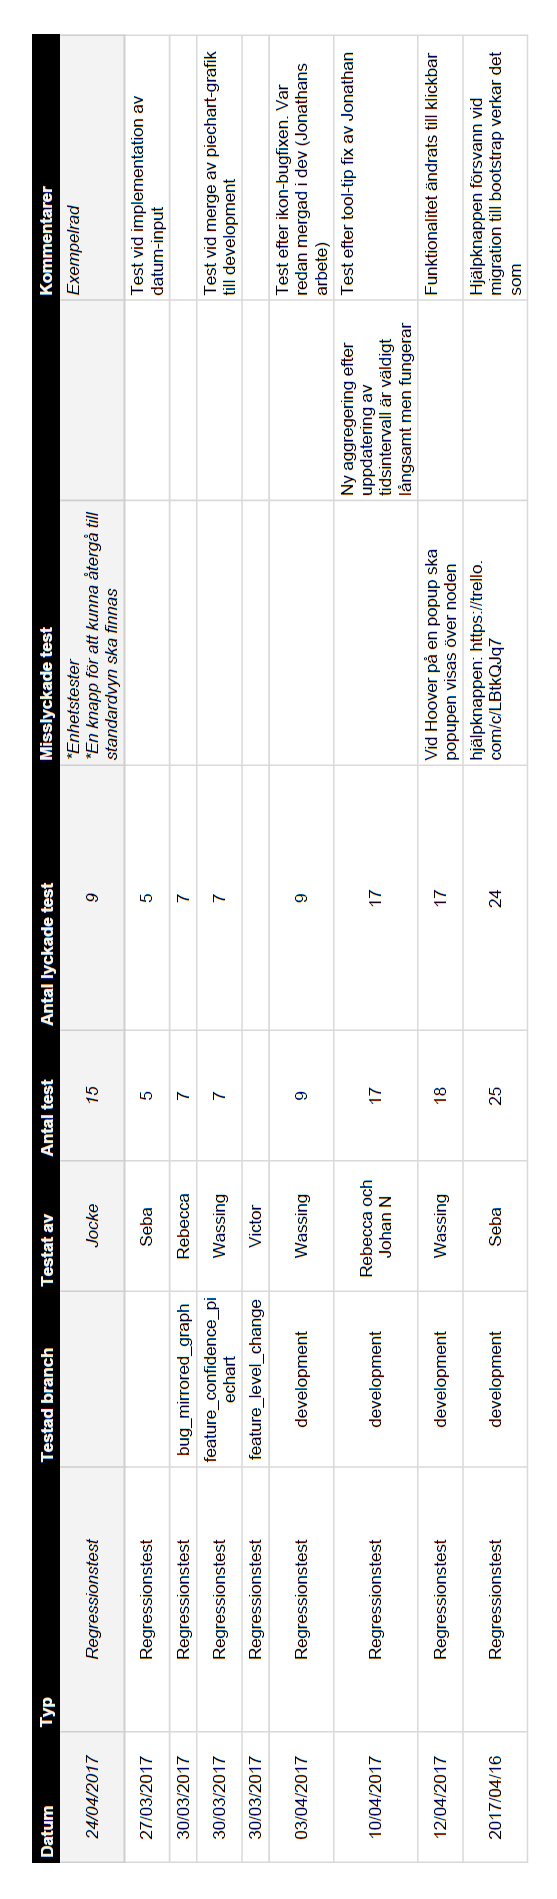
\includegraphics[scale=0.85]{log.png}

\newpage
%\section{Tillvägagångssätt}
I enlighet med agila utvecklingsmetoder behandlas testning likvärdigt med utvecklingsuppgifter och varje utvecklare väljer och utför dessa under utvecklingssprintens gång. \\
\subsection{Regressionstestning}
Regressionstestning utförs veckovis för att kunna säkerställa byggets status. Varje vecka tillsätts en utvecklare som är ansvarig för den veckans regressionstestning och testar då all tidigare implementerad funktionalitet tillsammans med den veckans nya funktionalitet. Som ett steg i regressionstestningen enhetstestas även tidigare funktionalitet genom ramverket Eiffels automatiska enhetstestning. När regressionstestning utförts registreras detta i databladet \textit{Dokumentation/Testning/Teststatus} för spårbarhet. Där noteras hur många tester som genomförts, antalet tester som ej godkändes och vilka det var. 
\\
\subsection{Enhetstestning}
Varje utvecklare är ansvarig för att skapa enhetstest för den funktionalitet som implementeras. Dessa enhetstester skapas för att fungera tillsammas med ramverket Mocha\cite{website:mocha} med tillägget Chai\cite{website:mocha} som en del av ramverket Meteor\cite{website:meteor}. 


\newpage
%\section{Kriterier för godkänd/misslyckat test}
För att ett test ska anses vara godkänt så måste det uppfylla testpåståendet enligt nedanstående standard för hur testfall och testpåståenden formuleras.
\subsection{Testfall}
\textbf{Påstående:} \textit{Vad som ska verifieras. Se nedan (Formulering av testpåstående).}\\
\textbf{Antaganden:} \textit{De antaganden som understödjer testfallet.}\\
\textbf{Testdata: } \textit{Variabler och värden som testas.}\\
\textbf{Teststeg: } \textit{Arbetsgång för testet.}\\
\textbf{Förväntat resultat: } \\
\textbf{Uppnått resultat: } \textit{Vad resulterade testet i.}\\
\textbf{Godkänt/Underkänt test:} \textit{Huruvida testet godkändes eller ej.}\\
\textbf{Kommentarer:} 
\subsection{Testpåstående}
För att formulera vad som ska verifieras används följande format: \\
\\
\textbf{Verifiera ...} \\
\textbf{... genom att använda ...} [verktyg, dialog] \\
\textbf{... med ...} [förutsättningar] \\
\textbf{... att ...} [vad som returneras, visas eller demonstreras]
\\ \\
För att testet ska betraktas som godkänt ska testet uppfylla följande kriterier:
\begin{itemize}
\item Testpåståendet är uppfyllt
\item Inga ytterligare antaganden är gjorda
\item Testdata har hämtats in
\item Teststegen har följts vid utförandet av testet
\item Det förväntade resultet har uppnåtts eller överträffats
\end{itemize}

\subsection{Exempel på korrekt formulerat testfall}
\textbf{Påstående:} Verifiera genom tidtagning med ramverkets tidtagninsfunktionalitet att hemsidan läses in på under två millisekunder. \\
\textbf{Antaganden:} Webbläsarens cacheminne är rensat. \\
\textbf{Testdata:} Uppmätt tid \\
\textbf{Teststeg:} Starta tidtagning, läs in hemsidan, läs av inläsningstiden. \textit{Alternativt: Se checklista i Trellokortet.} \\
\textbf{Förväntat resultat: } Hemsidans inläsningstid understiger två millisekunder. \\
\textbf{Uppnått resultat:} Hemsidan inläsningstid var en millisekund.\\
\textbf{Godkänd/Underkänt test: } GODKÄNT \\
\textbf{Kommentarer:} Testet är allmängiltigt för alla marknadsledande webbläsare. 
%\newpage
%\section{Kriterier för avbrytande och återupptagande av test}
Ett test ska avbrytas i händelse av att antagandena inte kan uppfyllas, ytterligare antaganden måste göras eller testdata inte kan avläsas. Om teststegen inte kan utföras eller har avvikits från måste testet avbrytas. 
\\
\\
Testning kan återupptas om utförandet går att isolera till de teststeg som finns definierade i testfallet och det går att verifiera att avvikelserna från teststegen inte påverkat utfallet på testet. I händelse av att ytterligare antaganden gjorts, och det inte går att utesluta att det kan påverka testets utfall så avbryts testet och får ej återupptas tills dess att alla antaganden följer specifikationerna i testfallet. 
\\
\\
Ett test som avbryts får normalt återupptas omedelbart vid nästa teststeg, och räknas då som \emph{en} testsession. I de fall ett test inte får återupptas utan måste startas om som en ny testsession framgår detta tydligt i testfallets kommentar.
\newpage
%\section{Testleverabler}
Följande leverabler igår i slutleveransen och används som underlag för att styrka krav- och kvalitetsuppfyllelse.
\begin{itemize}
\item Testplan
\item Testfall
\item Testskript
\item Testrapport
\item Teststandard
\end{itemize}

\newpage
%\section{Personal- och kompetensbehov}
För att kunna utföra testning inom ramarna för projektet så krävs kunskaper inom följande områden:
\begin{itemize}
\item Användbarhetstest
\item CI-system
\item Generella programmeringskunskapser
\end{itemize}
\newpage
%\section{Ansvarsområden}
Ansvaret för att formulera enhetstestning ligger på den utvecklare som är ansvarig för en viss bit kod. Testerna måste vara oberoende av varandra och inte vara beroende av resultatet från tidigare test. Enhetstesten testar enskild funktionalitet och jämför output från funktioner med förväntad output.\\
\\
Det ska eftersträvas att skriva testfall först och sedan metoden som ska implementeras. Detta gör det också tydligt när utvecklingen är klar. Manuell testning innan enhetstest skrivits är inte att föredra!\\
\\
Varje funktionalitet är kopplat till ett Trello-kort som representerar en aktivitet som ska utföras. Dessa aktiviteter testas genom att varje utvecklare tilldelar sig själv en aktivitet att testa likt de tilldelar sig själv aktiviteter för utveckling. Förutom enhetstester så testar ingen utvecklare funktionalitet som den har utvecklat. Detta görs för att säkerställa att testen utförs helt oberoende.
\newpage
%\section{Schema}
%\section{Planeringsrisker och beredskapsplan}

%... add more as needed
\clearpage
\printbibliography

\newpage
\begin{appendices}

\end{appendices}

\end{document}